\documentclass{scrartcl}			% defines the kind of document you want to produce

% Include different packages:
\usepackage[utf8x]{inputenc}
\usepackage[T1]{fontenc}
\usepackage{lmodern}
\usepackage[english]{babel}
\usepackage{amsmath}
\usepackage{graphicx}           	% include graphics
\usepackage{caption}	
\usepackage{subcaption}	 
\usepackage{hyperref}
\usepackage{epstopdf}
\usepackage{siunitx}
\usepackage{float}

\title{Neuroprothetics Exercise 8\\Noise Vocoder}
\author{ Laura Bielenberg }
\date{\today}

\begin{document} 					% Document begins here

\maketitle


\section{Noise vocoder with dynamic compression}
The code used to generate the following plots has been written using Python 3.7. Please run the  script \texttt{code/exercise\_8.py} to execute the code related to this exercise.

\subsection{Filtered noise}\label{sec:filtnoise}
The initial noise signal is generated from a zero-mean Gaussian distribution and has the same length $N$ as the audio input array. Thus each sample $x_i ... x_N$ of the noise signal follows:
\begin{equation}
	x_i \sim \mathcal{N}(0, 1) \text{ for } i \in \left\{1 .. N\right\} \, .
\end{equation}
Afterwards, the noise signal is band-pass filtered using the CI filter banks from exercise 7.
Figure~\ref{fig:noise} shows the filtered noise for a 12 channel CI filter bank. The reason the first two channels appear as flatlines, is because the signals have been normalised for the plots, and those two signals seem too have very high maximal amplitudes. This does not look intuitive to me and I suspect an issue with the filter bands due to the higher filter order.

\begin{figure}[H]
\centering
   		 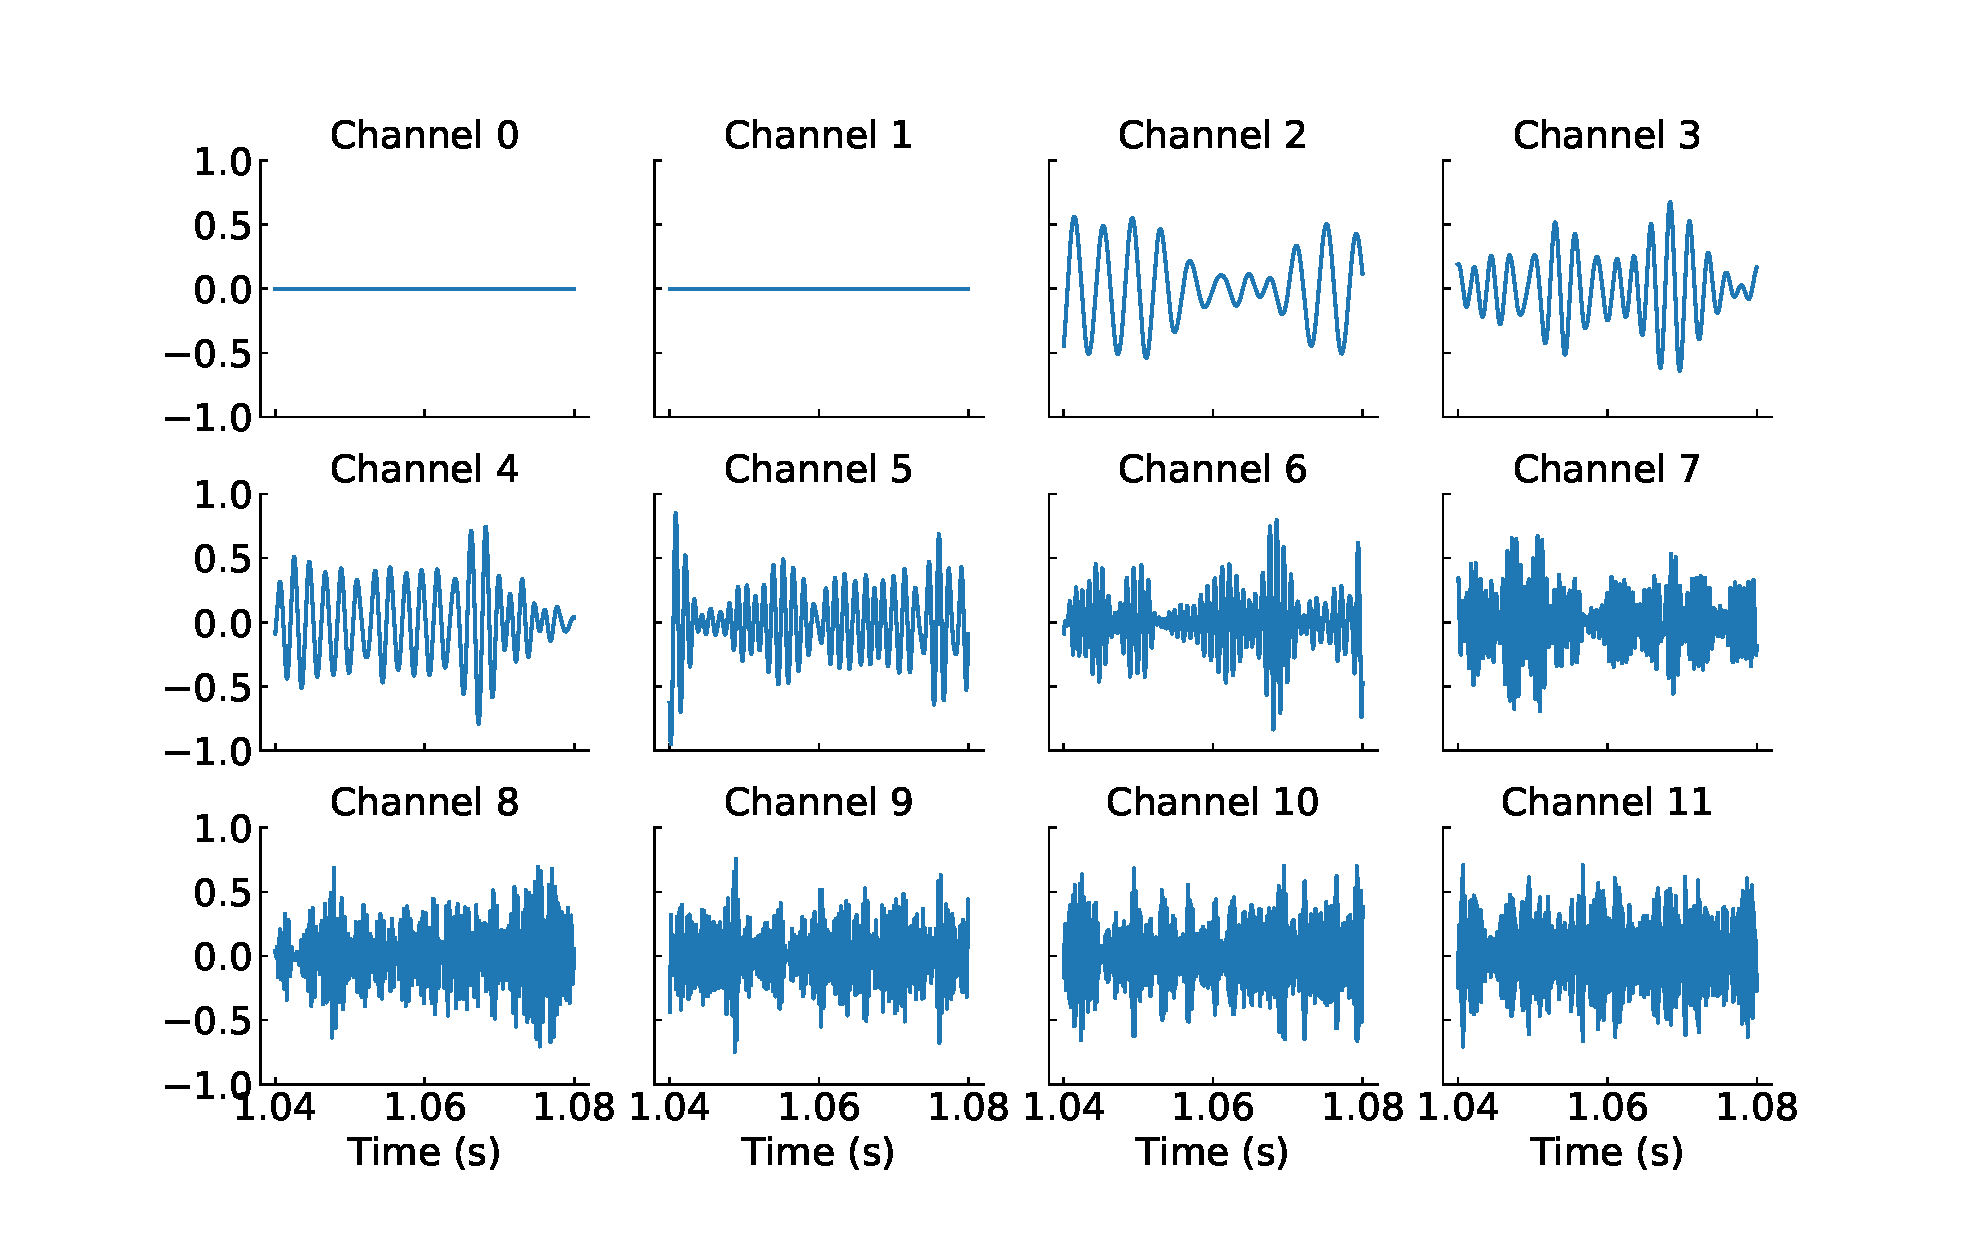
\includegraphics[width=\linewidth]{imgs/noise_filtered_timeslot.eps}
   		 \caption{Noise filtered by 12 CI filter bank.} 
   		 \label{fig:noise} 
\end{figure}

\subsection{Extract envelopes}
The audio signal used in this exercise is the same as in exercise seven. It is the word "sorekara", which was recorded with a sampling frequency $f_s=\SI{44100}{Hz}$. The signal array has an overall length of $N=107520$ samples.\\
This signal is filtered with a fourth order butterworth filter.
In order to extract the envelopes of the band-pass filtered electrode signals for this audio signal, the hilbert transform is used which creates the analytical signal 
\begin{equation}
s_A(t) = s(t) + j\hat{s}(t) .
\end{equation}
Since $s_A$ is complex valued it can be expressed in exponential notation as
\begin{equation}
s_A(t) = A(t)e^{j\psi(t)} 
\end{equation}
where $A(t)$ is the envelope (instantaneous amplitude) and $\psi(t)$ is the instantaneous phase.\\
\\
As the envelopes resulting from applying the hilbert transform alone are not very clear, I added a post-processing step in which the envelopes are being filtered by a butterworth low-pass with a cut-off frequency of $\SI{30}{Hz}$ such that the peaky behaviour of the higher frequencies was smoothed out.\\
Figure~\ref{fig:env} shows the original band-pass filtered electrode signals of a 12 electrode CI with their resulting envelopes.

\begin{figure}[H]
\centering
   		 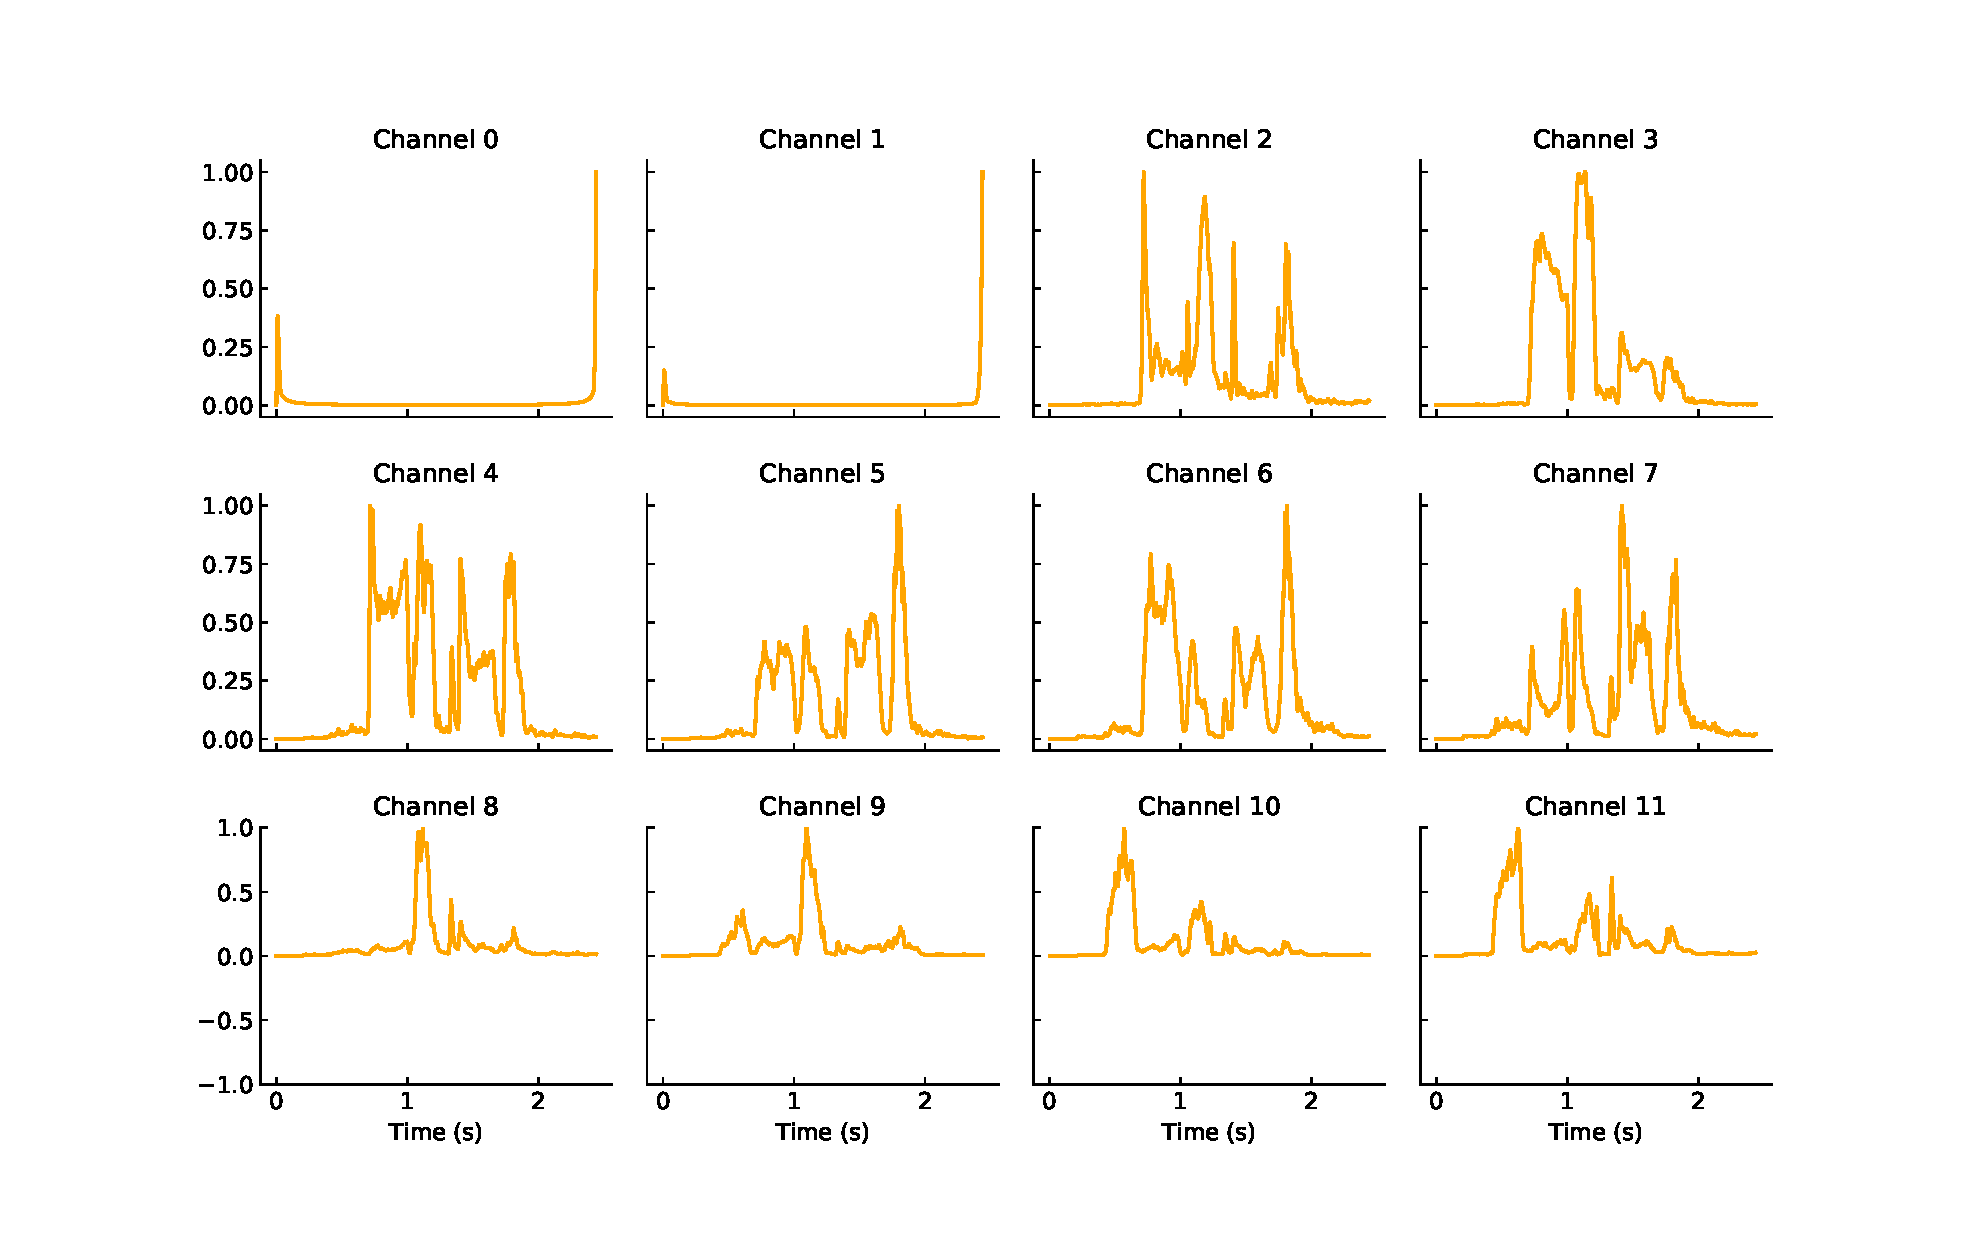
\includegraphics[width=\linewidth]{imgs/envelopes.eps}
   		 \caption{Envelopes (orange) of the band-pass filtered audio signal (blue) for a 12 electrode CI.} 
   		 \label{fig:env} 
\end{figure}

\subsection{Add dynamic compression}
In a further step, dynamic compression is applied to each of the extracted envelopes, mapping the envelopes to a logarithmic scale according to
\begin{equation}
env_{compressed}=\frac{log_{10}(1+c*env)}{log_{10}(c+1)}
\end{equation}
where $c$ denotes the compression rate which was set to $c=500$.\\
After the compression the signal is clipped by setting all values greater than one to one, as well as introducing a lower clipping threshold to set noise values below this threshold to zero.\\ 
The results for different lower clipping thresholds can be heard by executing the ecercise script at \texttt{code/exercise\_8.py}.\\ The result that cancels out most of the noise and still leaves a good signal is that with a threshold of $t_{lower}=0.6$. 

\subsection{Finalize the Vocoder}
In the end, the envelopes are multiplied by the respective band-limited noise and the single channels are summed up.\\Playing back the sound shows that it is quite noisy, but it can still be understood what is being said. Figure~\ref{fig:dyn} shows the corresponding vocoder output, which corresponds to the spectrum of the summed output signal on a loglog scale. Figure~\ref{fig:ci_12_spec} shows the spectrogram for the uncompressed 12 CI electrode from exercise seven, while figure~\ref{fig:ci_12_spec_clip} shows the spectogram of the summed and commpressed vocoder output for a $c=500$ and $t_{thresh}=0.6$. Both are plottet using a time window of 10 ms and an overlap of 5 ms. It can be seen that the overall noise level is increased when using dynamic compression. Also, the understandability of the spoken word decreases, which can also bee seen in the plots.
\begin{figure}[H]
\centering
   		 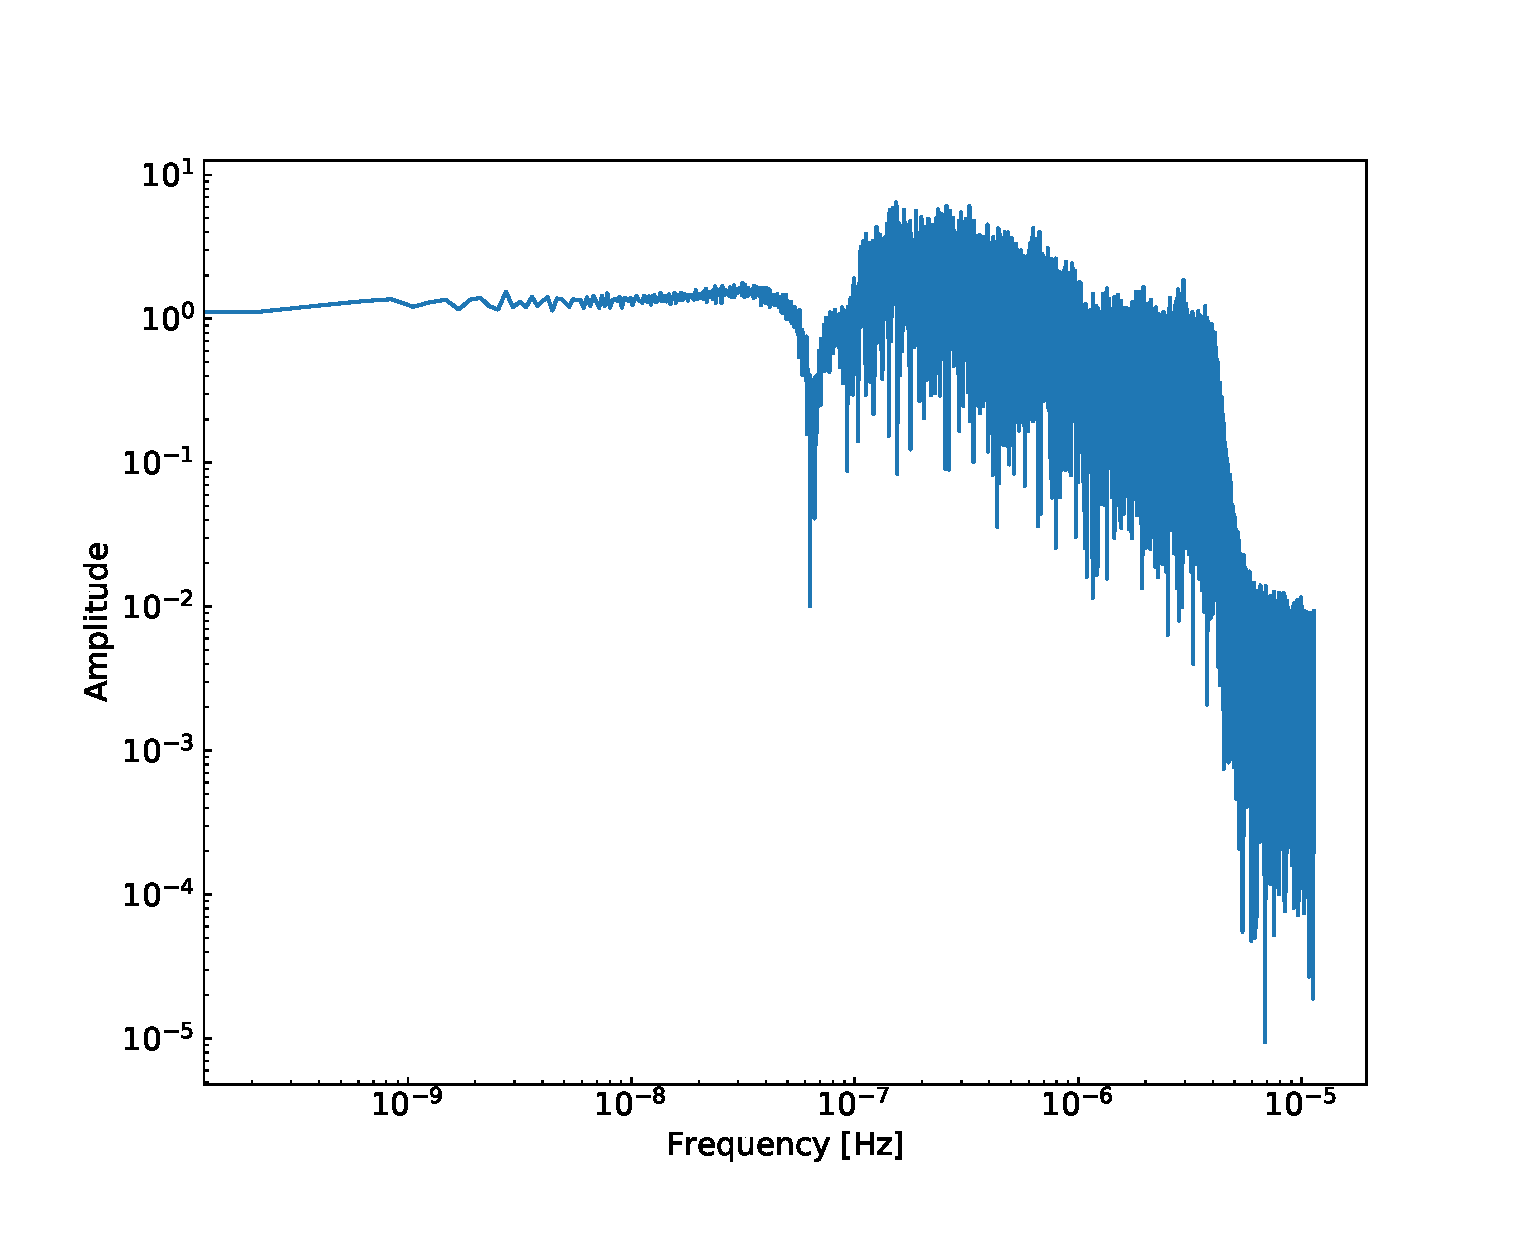
\includegraphics[width=\linewidth]{imgs/vocoder_lower_clip_06.eps}
   		 \caption{Compressed vocoder output for $c=500$ and $t_{lower}=0.6$.} 
   		 \label{fig:dyn} 
\end{figure}
\begin{figure}[H]
\centering
   		 \includegraphics[width=0.8\linewidth]{../tex_7/imgs/spectogram_12_CI.eps}
   		 \caption{Spectogram for a 12 electrode CI from exercise 7.} 
   		 \label{fig:ci_12_spec} 
\end{figure}
\begin{figure}[H]
\centering
   		 \includegraphics[width=0.9\linewidth]{imgs/spectogram_vocoder_lower_clip_06_CI.eps}
   		 \caption{Spectogram for a 12 electrode CI with $c=500$ and $t_{lower}=0.6$ .} 
   		 \label{fig:ci_12_spec_clip} 

\end{figure}

\end{document}
